\subsection{Idea and background}
\thomas{This section seems to repeat (technically this is the first occurence) information that will be mentioned at least 2 more times in later chapters - if it is meant as a brief resume it should be revised! Otherwise deleted.}
This section briefly covers a description of the problem that we are trying to solve, how we are going to solve it, which customers that could have an interest in it and how we would benefit from it and create profit.

It will also contain a short presentation of members of the team and an explanation as to why we are the perfect fit for this start up company.

\subsubsection{Problem}
The problem that we seek to solve involves flexibility within the area of industrial manufacturing. Usually a recipe is made and stored for each individual task.
Making these recipes, or reprogramming the robots is necessary whenever a new task arises and within parts of the manufacturing business this is a common occurance. 
Adaptability and precision are major keywords when it comes to welding tasks for industrial robots. Both adjectives that do not describe current methods well.

\subsubsection{Solution}
We provide a solution to the problem mentioned above, which does not require programming. The product itself is an add-on for welding robots, that allows the robot to detect welding seams with minimal user interaction. The add-on will provide coordinates, used to create a welding-path for the robot. 

The product consists of a micro computer, which is used to make calculations based on input from a camera and a laser range scanner. 

\subsubsection{Customer}
Relevant customers are companies who are already in the zone of robotic welding, companies who could be interested in buying the product to supplement their own products. Primarily it will be customers who develop either robots or other technical parts for them.  

\subsubsection{Revenue}
A revenue stream is generated through the sales channel to the various robot-developing companies, who end up providing the product to the end customers.
We will develop our product for specific welding robots for a price, providing another potential revenue stream. 
Patenting the product will be also an important part to maintain revenue, as it will allow us to charge a significant sum of money from companies who wish to use our technology.

\subsubsection{The Team}
We are a dedicated team of engineering students. We believe that we have the necessary drive and expertise to realise this project. This project is an extension of our individual interests and as such it is only natural that we extend this to our proffesional careers. Below is a presentation of all of the members of the team.

\begin{table}[h]
\centering
\begin{tabular}{|c|c|c|c|}
\hline
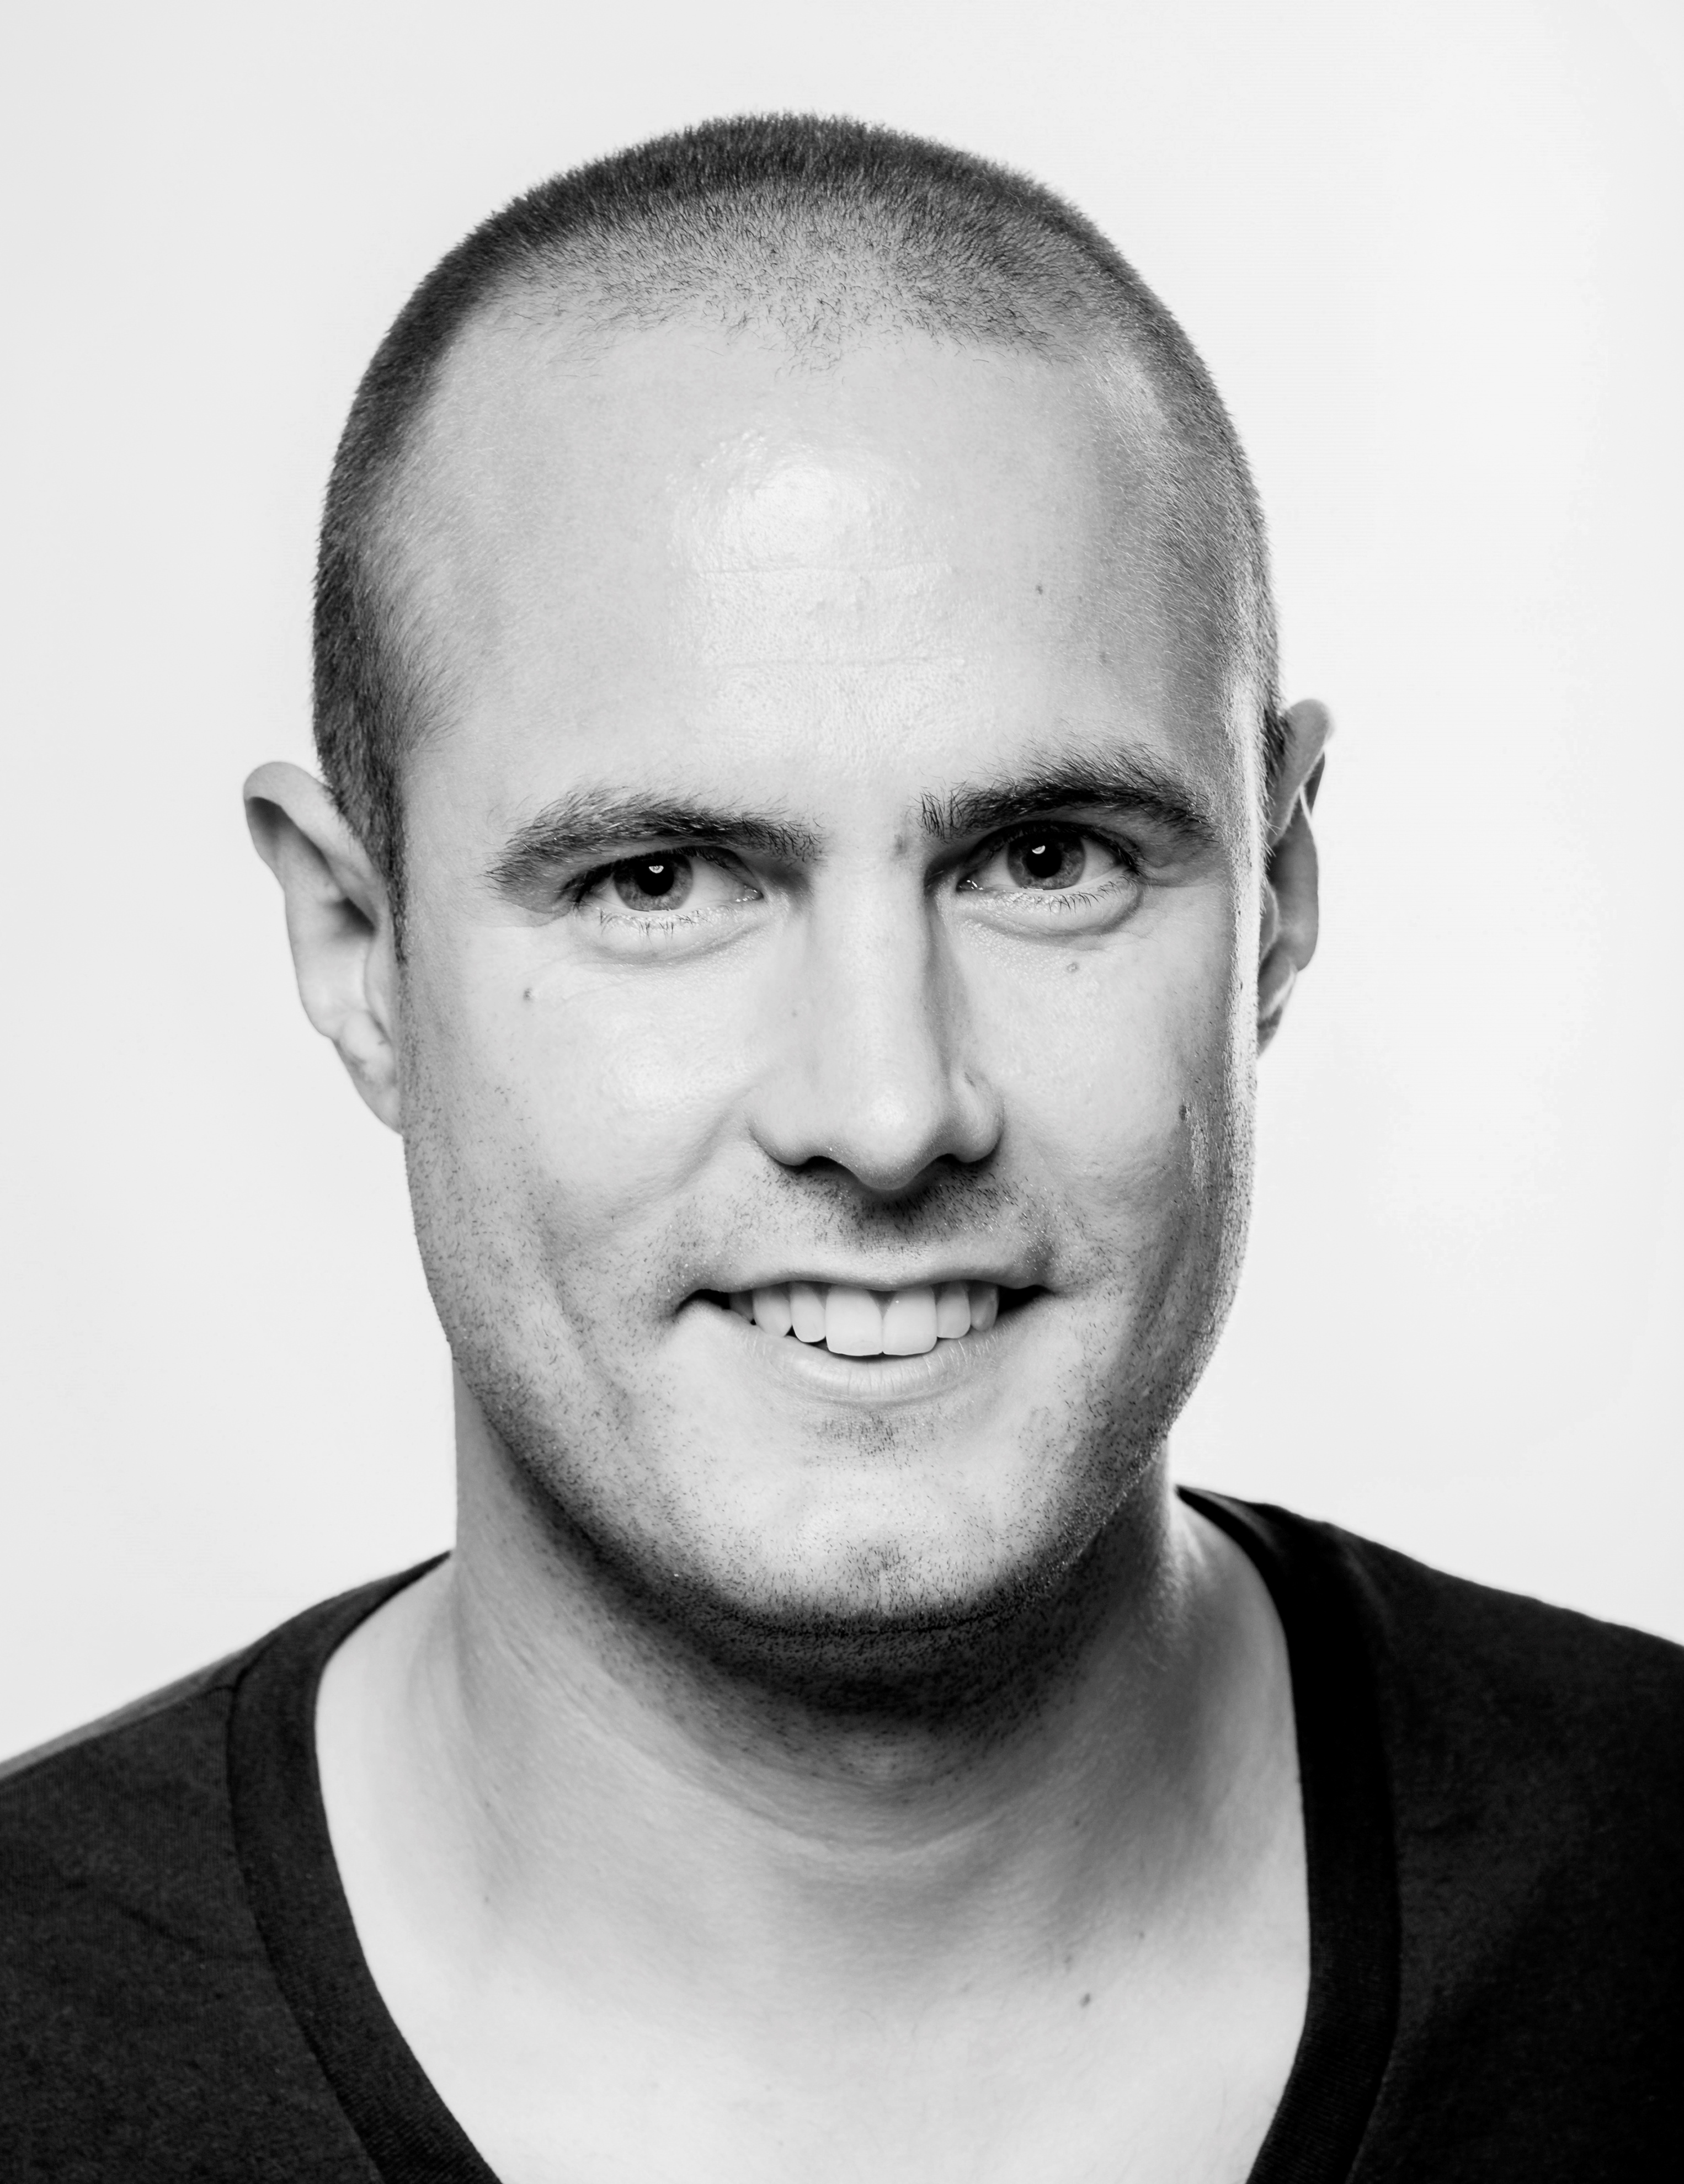
\includegraphics[width=0.2\textwidth]{graphics/cgopic} & %casper

\includegraphics[width=0.2\textwidth]{graphics/AnonProfile} & %david

\includegraphics[width=0.2\textwidth]{graphics/AnonProfile} & %kirstine

\includegraphics[width=0.2\textwidth]{graphics/Nikolaj_profile} \\ \hline %nikolaj
\parbox[t] {0.2\textwidth}{
\textbf{Casper:} \\
28 years old, originally from Gelsted, Denmark. Educated Electrician. Studying Energy Technology.
}

&

\parbox[t] {0.2\textwidth}{
\textbf{David:} \\

} 

&

\parbox[t] {0.2\textwidth}{
\textbf{Kirstine:} \\

} 

&

\parbox[t] {0.2\textwidth}{
\textbf{Nikolaj:} \\
I am 24 years old and originally from Esbjerg, Denmark. I am currently studying M.Eng in Robotic Systems.
} 

\\\hline
\end{tabular}

\begin{tabular}{|c|c|c|}
\hline
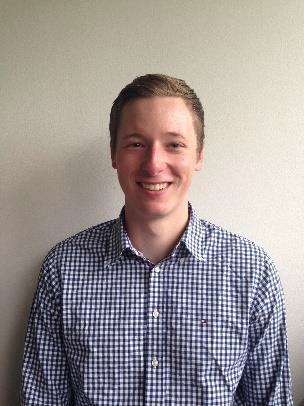
\includegraphics[width=0.215\textwidth]{graphics/Simon_profile} & %simon

\includegraphics[width=0.2\textwidth]{graphics/AnonProfile} & %thomas
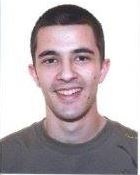
\includegraphics[width=0.2\textwidth]{graphics/sexy_xabi_profile} \\ \hline %xabier
\parbox[t] {0.2\textwidth}{
\textbf{Simon:} \\
I am 23 years old and originally from Haderslev, Denmark. Currently studying IT-Engineering.

} 

&

\parbox[t] {0.2\textwidth}{
\textbf{Thomas:} \\
Age: 26, from Tønder. I'm currently studying to become M.Eng in Robotic Systems
} 

&

\parbox[t] {0.2\textwidth}{
\textbf{Xabier:} \\
I am 21 years old and originally from Bilbao, Spain. I am currently studying Industrial Engineering.
} 

\\\hline
\end{tabular}
\end{table}



\subsubsection{Passion}
With a team profile that covers most roles, the group is well balanced. One of our main strengths is the analytical skills and assets of our specialists, which form more than half of the team.  
With skills such as programming, knowledge within the field of robots, software designing and lasers, each development challenge is right within our area of expertise. 
Our motivation is the very real possibility that we will create a product that will provide the industry, not only with a highly flexible welding solution, but also the basis for an entirely new application of existing technologies that could be employed in many other industries.
It is our conviction that we are the right team to bring together this range of technologies to create something new, exiting and potentially highly lucrative.